%%%%%%%%%%%%%%%{fontspec}%%%%%%%%%%%%%%%
%将no-math选项传递给fontspec宏包,该选项禁用了使用fontspec宏包中的数学字体功能。
\PassOptionsToPackage{no-math}{fontspec}
%%%%%%%%%%%%%%%{xeCJK}%%%%%%%%%%%%%%%
%将AutoFakeBold和AutoFakeSlant选项传递给xeCJK宏包,这两个选项让xeCJK宏包自动产生伪粗体和伪斜体效果。
\PassOptionsToPackage{AutoFakeBold=true,AutoFakeSlant=true}{xeCJK}

\documentclass{book}
\usepackage[heading=true
,scheme=chinese%中文方案
,fontset=none%不使用默认的字体设置
,space=auto%自动调整中英文间距
]{ctex}
\setCJKmainfont{方正书宋_GBK}%方正书宋_GBK.TTF  设置文本的中文有衬线字体为“方正书宋_GBK”
\setCJKsansfont{方正黑体简体}%方正黑体_GBK.TTF  设置文本的中文无衬线字体为“方正黑体简体”
\setCJKmonofont{方正书宋简体}%方正仿宋_GBK.TTF  设置文本的中文等宽字体为“方正书宋简体”

\usepackage{newclude}%后面 \include* 引用就不会自动分页了
%\includeonly{1}%加上这句,就只有1的两个引入有效果了

\makeatletter
\providecommand*\input@path{}
\newcommand*\addinputpath[1]{\expandafter\def\expandafter\input@path\expandafter{\input@path#1}}
\makeatother

\addinputpath{%
{/Users/virhuiai/hlProjects/Latex-Typesetting-Hub/练习书本排版/iText_in_Action_Second_Edition}%
}

\usepackage[all]{tcolorbox}
% \tcbuselibrary{documentation}

\begin{document}


%%%sumBgColor%%%%%%%%%%%%%%%%%%%%%%%%%%%%%%%%%%%%%%%%%%%%%%%%%%%%%%%%%%%%%%%%%
%abstractlist
\definecolor{sumBgColor}{RGB}{236, 236, 211}
\definecolor{sumTxtColor}{RGB}{167, 33, 22}
\newenvironment{itemizeSum}{%
\begin{itemize}}{\end{itemize}}
\tcolorboxenvironment{itemizeSum}{
%before skip和after skip选项分别表示在环境前后添加6pt的垂直空白。
% before skip=6pt,after skip=6pt,
breakable,%
opacityframe=0.0,colback=sumBgColor,colupper=sumTxtColor,grow to left by=2em,before upper={\textbf{This chapter covers\\本章涵盖了}}
}
%%%%%%%%%%%%%%%%%%%%%%%%%%%%%%%%%%%%%%%%%%%%%%%%%%%%%%%%%%%%%%%%%%%%

\newtcolorbox[blend into=figures]{myfigure}[2][]{float=htb,capture=hbox,
title={#2},every float=\centering,#1}
     
% \include*{Creating_PDF_documents_from_scratch/Creating_PDF_documents_from_scratch}%不会分页
%%chapter1:Creating_PDF_documents_from_scratch
% \include*{Creating_PDF_documents_from_scratch/Introducing_PDF_and_iText/Introducing_PDF_and_iText}%不会分页
% 1.1
\setcounter{chapter}{1}
\section{Things you can do with PDF\\PDF的用途}

Let’s start with six quick facts about PDF:\\让我们从六个关于PDF的快速事实开始:

\begin{itemize}
\item
PDF is the Portable Document Format.\\PDF是可移植文档格式。

\item
It’s an open file format (ISO-32000-1), originally created by Adobe.\\它是一个开放的文件格式(ISO-32000-1),最初由Adobe创建。

\item
It’s used for documents that are independent of system software and hardware.\\它用于独立于系统软件和硬件的文档。

\item
PDF documents are an essential part of the web.\\PDF文档是Web的关键部分。

\item
Adobe Reader is the most widely used PDF viewer.\\Adobe Reader是最广泛使用的PDF阅读器。

\item
There are a lot of free and proprietary, open and closed source, desktop and web-based software products for creating, viewing, and manipulating PDF documents.\\有许多免费和专有的、开放和闭源的、桌面和基于Web的软件产品,用于创建、查看和操作PDF文档。\end{itemize}

Figure \ref{fig:PDF相关功能概述} offers an overview of the things you can do with PDF. There are tools to create PDF documents, there are applications to consume PDF documents, and there are utilities to manipulate existing PDF documents.

图 \ref{fig:PDF相关功能概述} 提供了关于使用PDF所能做的事情的概述。有用于创建PDF文档的工具,有用于消费PDF文档的应用程序,还有用于操作现有PDF文档的实用程序。

% Figure 1.1 Overview of
% PDF-related functionality.
% The functionality covered
% by iText is marked with
% the iText logo.
\begin{myfigure}{PDF相关功能概述。iText涵盖的功能标有iText标志。\label{fig:PDF相关功能概述}}
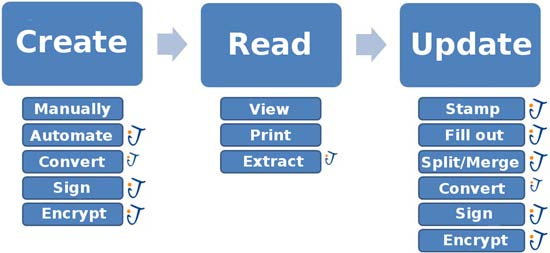
\includegraphics[height=4cm]{/Users/virhuiai/hlProjects/Latex-Typesetting-Hub/练习书本排版/iText_in_Action_Second_Edition/Creating_PDF_documents_from_scratch/Introducing_PDF_and_iText/index-35_1.jpg}
\end{myfigure}

% 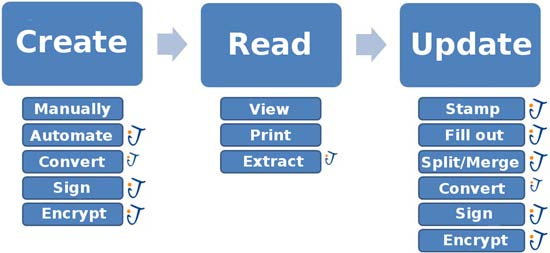
\includegraphics[height=4cm]{/Users/virhuiai/hlProjects/Latex-Typesetting-Hub/练习书本排版/iText_in_Action_Second_Edition/Creating_PDF_documents_from_scratch/Introducing_PDF_and_iText/index-35_1.jpg}

If you look at PDF creation, you’ll find that graphical designers use desktop applications such as Adobe Acrobat or Adobe InDesign to create a document in a manual or semimanual process. In another context, PDF documents are created programmatically, using an API to produce PDFs directly from software applications, without—--or with minimal—human intervention. Sometimes the document is created in an inter-mediary format first, then converted to PDF. These different approaches demand different software products. The same goes for PDF manipulation. You can update a PDF
manually in Adobe Acrobat, but there are also tools that allow forms to be filled out automatically based on information from a database.

如果您看PDF的创建,您会发现图形设计师使用桌面应用程序,如Adobe Acrobat或Adobe InDesign,以手动或半自动的方式创建文档。在另一种情况下,使用API从软件应用程序直接生成PDF,而不需要或只需要最少的人工干预。有时文档首先以中介格式创建,然后转换为PDF。这些不同的方法需要不同的软件产品。对于PDF操纵也是如此。您可以在Adobe Acrobat中手动更新PDF,但也有工具可以根据来自数据库的信息自动填写表格。

\end{document}
%cd /Volumes/RamDisk/ &&  xelatex --output-directory=/Volumes/RamDisk/ -synctex=1 -shell-escape  /Users/virhuiai/hlProjects/Latex-Typesetting-Hub/练习书本排版/iText_in_Action_Second_Edition/iText_in_Action_Second_Edition.tex